Das erste Experiment dieser Reihe bietet vergleichsweise viel Platz. Es ist vor allem für den späteren Vergleich interessant.

\textbf{Aufbau des Experiments}
\begin{figure}[H]
    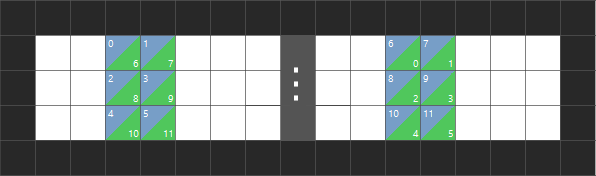
\includegraphics[width=\textwidth]{images/6vs6_spacy.png}
    \centering
    \caption{Aufbau für die lockere Vorbeifahrt zweier Gruppen, bestehend aus jeweils sechs Agenten}
    \label{fig:6x6Locker}
\end{figure}
 Die Abbildung \ref{fig:6x6Locker} zeigt eine Karte die drei mal 30 Felder misst. Es stehen sich zwei Gruppen, bestehend aus jeweils sechs Agenten, gegenüber. Zum rechten beziehungsweise linken Rand sind für die Gruppen noch ein paar freie Felder vorhanden. Damit soll es den Agenten möglich sein, Ausweichbewegungen nach hinten hin ausführen zu können.